\documentclass{article}

\usepackage{graphics}
\usepackage[vcentering]{geometry}

\geometry{papersize={9.25in,2.4in}, top=0.05in, bottom=0in, left=0in, right=0in}

\usepackage{tikz}
\usetikzlibrary{
	arrows,shapes,decorations.pathmorphing,backgrounds,positioning,fit,calc,scopes
}
\tikzset{
  auto,
  compartment/.style={
    rectangle, minimum size=9mm, rounded corners=2mm,
    thick, draw=black!15, top color=white,bottom color=black!30
  },
  %
  bigcompartment/.style={
    rectangle, minimum size=20mm, rounded corners=2mm,
    thick, draw=black!30, top color=white,bottom color=black!20
  },
  %
  point/.style={
    circle, inner sep=2pt, fill=black!5
  },
  %
  mytextbox/.style={
    rectangle, text=black!50, thin, 
    draw=white, top color=white,bottom color=white, fill=white
  }
}


% \definecolor{c1}{RGB}{217, 95, 2}
% \definecolor{c2}{RGB}{117, 112, 179}
% \definecolor{c3}{RGB}{231, 41, 138}
% \definecolor{c4}{RGB}{102, 166, 30}

\definecolor{localc}{RGB}{236, 175, 100}
\definecolor{effc}{RGB}{186, 184, 217}
\definecolor{obsc}{RGB}{243, 148, 197}
\definecolor{intc}{RGB}{153, 209, 89}

\usetikzlibrary{arrows.meta}

\begin{document}

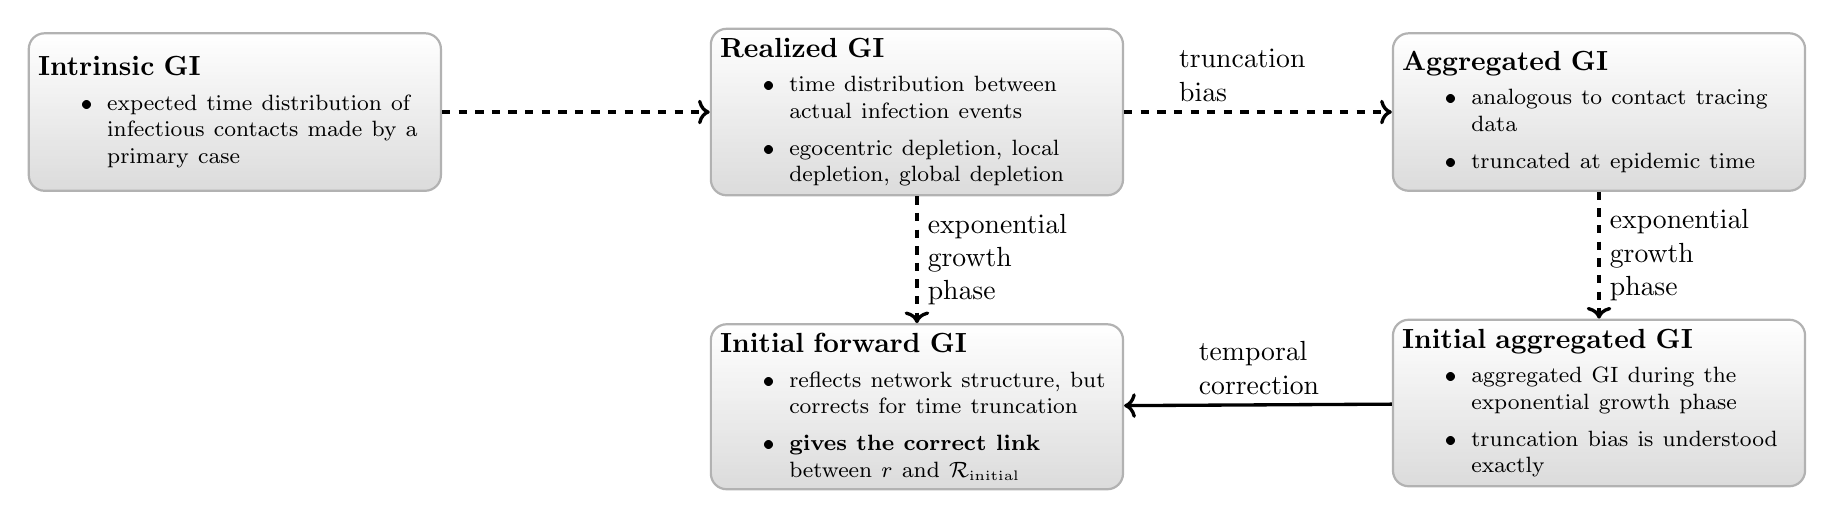
\begin{tikzpicture}
\node(int)[bigcompartment, text width=5cm, fill opacity=0.7, text opacity=1]{
    \textbf{Intrinsic GI}
    \footnotesize{
        \begin{itemize}
        \item expected time distribution of infectious contacts made by a primary case
        \end{itemize}
    }
};

\node(local)[bigcompartment, right=3.4cm of int, text width=5cm, fill opacity=0.7, text opacity=1]{
    \textbf{Realized GI}
    \footnotesize{
        \begin{itemize}
        	\item time distribution between actual infection events
        	\item egocentric depletion, local depletion, global depletion
        \end{itemize}
    }
};

\node(forward)[bigcompartment, below=1.61cm of local, text width=5cm, fill opacity=0.7, text opacity=1]{
    \textbf{Initial forward GI}
    \footnotesize{
        \begin{itemize}
        	\item reflects network structure, but corrects for time truncation
        	\item \textbf{gives the correct link} between $r$ and $\mathcal{R}_{\textrm{\tiny initial}}$
        \end{itemize}
    }
};

\node(agg)[bigcompartment, right=3.4cm of local, text width=5cm, fill opacity=0.7, text opacity=1]{
    \textbf{Aggregated GI}
    \footnotesize{
        \begin{itemize}
        	\item analogous to contact tracing data
        	\item truncated at epidemic time
        \end{itemize}
    }
};

\node(iniagg)[bigcompartment, below=1.61cm of agg, text width=5cm, fill opacity=0.7, text opacity=1]{
    \textbf{Initial aggregated GI}
    \footnotesize{
        \begin{itemize}
        	\item aggregated GI during the exponential growth phase
        	\item truncation bias is understood exactly
        \end{itemize}
    }
};
\draw[->, very thick, dashed] (int) -- node [midway, left, text width=2cm, align=right] {} (local);
\draw[->, very thick, dashed] (local) -- node [midway, right, text width=2cm] {exponential growth \\ phase} (forward);
\draw[->, very thick, dashed] (local) -- node [midway, above, text width=2cm] {truncation \\ bias} (agg);
\draw[->, very thick, dashed] (agg) -- node [midway, right, text width=2cm] {exponential growth \\ phase} (iniagg);
\draw[->, very thick] (iniagg) -- node [midway, above, text width=1.5cm] {temporal \\ correction} (forward);

\end{tikzpicture}

\end{document}
